\documentclass{ctexart}
\usepackage{tikz}
\usetikzlibrary{arrows, decorations.pathmorphing, backgrounds, positioning, fit, petri, automata}
\definecolor{yellow1}{rgb}{1,0.8,0.2}

\author{xzx}
\title{assignment3我的答案}


\begin{document}
\maketitle
\setcounter{page}{0}
\thispagestyle{empty}
\newpage

\begin{flushleft}



\section{Q1: Image Captioning with Vanilla RNNs}


\subsection{Recurrent Neural Networks}
首先是单个神经元的前向与后向传播。一个神经元的示意图如图
\ref{fig:rnn_step_forward}所示.

\begin{figure}[h]


  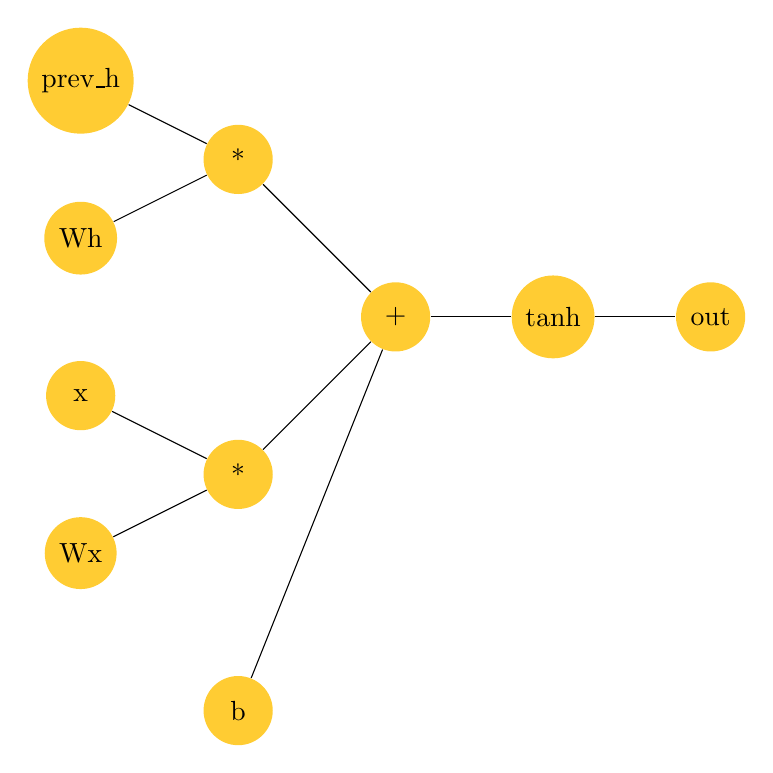
\begin{tikzpicture}
    \tikzstyle{every state} = [fill=yellow1,draw=none,text=black]
    \node[state] (p_h)             at (-4,8) {prev\_h};
    \node[state] (wh)              at (-4,6) {Wh};
    \node[state] (x)               at (-4,4) {x};
    \node[state] (Wx)              at (-4,2) {Wx};
    \node[state] (b)               at (-2,0) {b};
    \node[state] (mul1)            at (-2,7) {*};
    \node[state] (mul2)            at (-2,3) {*};
    \node[state] (add)             at (0,5)  {+};
    \node[state] (tanh)            at (2,5)  {tanh};
    \node[state] (out)             at (4,5)  {out};

    \path (p_h)     edge              node {}  (mul1)
          (wh)      edge              node {}  (mul1)
          (x)       edge              node {}  (mul2)
          (Wx)      edge              node {}  (mul2)
          (mul1)    edge              node {}  (add)
          (mul2)    edge              node {}  (add)
          (b)       edge              node {}  (add)
          (add)     edge              node {}  (tanh)
          (tanh)    edge              node {}  (out);

  \end{tikzpicture}
\caption{rnn\_step\_forward}
\label{fig:rnn_step_forward}
\end{figure}

反向传播也很容易根据这个图示推导出来.\\
整个rnn的前向与后向传播再课程里面已经把图给话出来了。这里面Wh 还有Wx被重复使用了很多遍。
对于一个变量后分成多条路径的,把这几条路径上面的微分相加。

\subsection{RNN for image captioning}
rnn的输入有点多,看上去有些混乱,整理一下输入放在图\ref{fig:rnn for image captioning}
中可以看的清楚一些。以图
\ref{fig:rnn_sample_input}为例作为输入.
\begin{figure}
  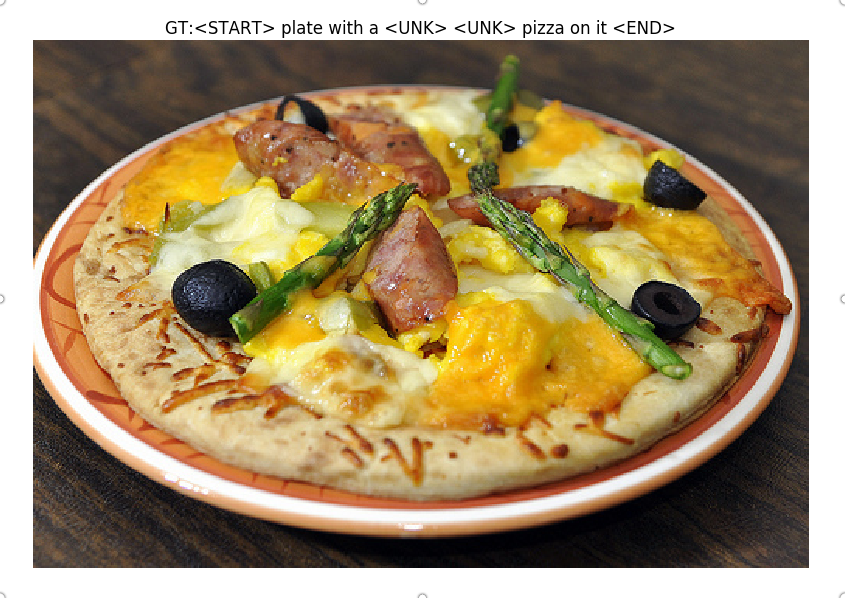
\includegraphics[width=5in]{./assignment1_pic/rnn_caption_sample.png}
  \caption{sample\_input}
  \label{fig:rnn_sample_input}
\end{figure}

\begin{figure}
  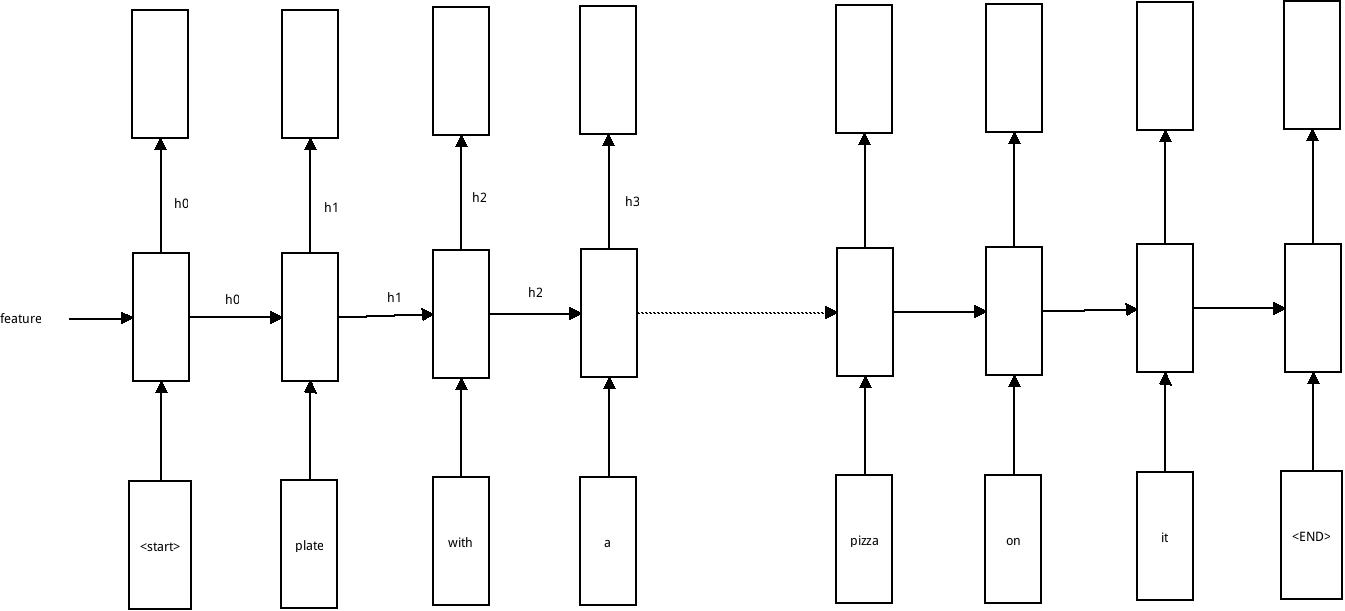
\includegraphics[width=5in]{./assignment1_pic/rnn_caption_train.jpg}
  \caption{RNN for image captioning}
  \label{fig:rnn for image captioning}
\end{figure}

每个神经元的输出会同时传给下个神经元并且向上传到上一层网络。这个ipynb的最开始就说已经帮我们
把图像的特征提取出来了,因此feature当做最初的h0传入网络就好了。每个单词对应的向量作为x从下面
输入到网络。











\end{flushleft}


\end{document}
